%volby: 
% male × female
% czech × english (zatím funguje jen czech)
% a studijní program / obor 
% is_bc (nejvíc odladěno)
% api_bc
% api_ing
% edu_bc
% edu_ing

\documentclass[male,czech,api_ing]{thesis}
\usepackage{ifthen}

\usepackage{amsmath,amssymb}
\usepackage{graphics}
\usepackage{color}
\usepackage{array}
\usepackage{longtable}
\usepackage{afterpage}
\usepackage{microtype}  % přesnější typografie
\usepackage{xcolor}
\usepackage{graphicx}

% Algorithms
\usepackage{algorithm}
\usepackage{algpseudocode}
\makeatletter
\renewcommand{\ALG@name}{Algoritmus}
\makeatother

\graphicspath{ {./images/} }

\usepackage{float}

% workaround for imcompatibility of czech babel and biblatex

\iftutex
\else
\usepackage{etoolbox}
\makeatletter
\newcommand\my@hyphen{-}
\newcommand\my@apostroph{'}
\patchcmd\select@language{-}{\my@hyphen }{}{}
\patchcmd\select@language{'}{\my@apostroph }{}{}
\makeatother
\fi

% fonty lze měnit (detaily viz sekce fonty)
\iftutex
	\usepackage{fontspec}  % nastavení fontů pro LuaLaTeX a XeLaTeX
	\setmainfont{Libertinus Serif}
	\setsansfont{Libertinus Sans}
	\setmonofont[Scale=MatchLowercase]{Libertinus Mono}
	\usepackage{unicode-math}
	\setmathfont{Libertinus Math}
\else
	\usepackage[utf8]{inputenc} % nastavení pro PDF LaTeX
	\usepackage[T1]{fontenc}
	\usepackage{libertinus}
	\renewcommand{\ttdefault}{pxtt}
\fi

\usepackage[style=iso-numeric,shortnumeration=true]{biblatex}
\addbibresource{thesis.bib}

\usepackage{csquotes} % uvozovky

% sazba ukázek kódu 

\usepackage{listings}
\renewcommand{\lstlistingname}{Ukázka kódu}

\lstdefinestyle{DOS}
{
    basicstyle=\scriptsize\color{black}\ttfamily,
    breaklines=true,
}

% ukázka pro nastavení balíku listings pro sazbu ukázek zdrojových kódů
\lstset{
  language=Python,                % the language of the code
  basicstyle=\small\ttfamily,    
  backgroundcolor=\color{white},   % choose the background color. You must add \usepackage{color}
  showspaces=false,                % show spaces adding particular underscores
  showstringspaces=true,           % underline spaces within strings
  showtabs=false,                  % show tabs within strings adding particular underscores
  frame=single,                    % adds a frame around the code
  tabsize=3,                       % sets default tabsize to 2 spaces
  breaklines=true,                 % sets automatic line breaking
  breakatwhitespace=false,         % sets if automatic breaks should only happen at whitespace
  keywordstyle=\bfseries,          % keyword style
  commentstyle=\rmfamily,       % comment style
  stringstyle=\itshape\color,   % string literal style
}

\definecolor{bluekeywords}{rgb}{0.13,0.13,1}
\definecolor{greencomments}{rgb}{0,0.5,0}
\definecolor{redstrings}{rgb}{0.9,0,0}

\lstset{
    language=[Sharp]C,
    showspaces=false,
    showtabs=false,
    breaklines=true,
    frame=single,
    tabsize=3,
    showstringspaces=false,
    breakatwhitespace=true,
    escapeinside={(*@}{@*)},
    commentstyle=\color{greencomments},
    keywordstyle=\color{bluekeywords}\bfseries,
    stringstyle=\color{redstrings},
    basicstyle=\small\ttfamily,
    numbers=left
}

% sazba matematických výrazů
% \newenvironment{conditions}[1][kde:]
%     {#1 \begin{tabular}[t]{>{$}l<{$} @{${}={}$} l}}
%     {\end{tabular}\\[\belowdisplayskip]}

\newenvironment{conditions}[1][kde:]
    {#1 \begin{tabular}[t]{>{$}l<{$} @{${}={}$} >{\raggedright\arraybackslash}p{10cm}}}
    {\end{tabular}}

% barevné zvýraznění textů, které je nutno nahradit
\newcommand{\ZT}[1]{\colorbox{yellow}{\color{red}{#1}}}


% TOTO JE POTŘEBA ZMĚNIT !!!!!!
\newcommand{\nazevcz}{Vliv předzpracování obrazu a augmentace dat na segmentaci rentgenových snímků}        % zde VYPLŇTE český název práce (přesně podle zadání!)
\newcommand{\nazeven}{Impact of image preprocessing and data augmentation on segmentation of X-ray images}     % zde VYPLŇTE anglický název práce (přesně podle zadání!)
\newcommand{\autor}{Bc. Milan Gittler}           % zde VYPLŇTE své jméno a příjmení
\newcommand{\rok}{\the\year}                
\newcommand{\vedouci}{RNDr. Jíří Škvára, Ph.D.}         
% zde VYPLŇTE jméno a příjmení vedoucího práce, včetně titulů
\newcommand{\vedouciDAT}{RNDr. Jiřímu Škvárovi, Ph.D.}   
% zde VYPLŇTE jméno a příjmení vedoucího práce, včetně titulů ve třetím pádě
                                                           
% zvětšuje o 23% vertikální okraje v tabulkách
\renewcommand{\arraystretch}{1.23}

% nastavení pro záhlaví (co nelze udělat v cls souboru)
\renewcommand{\chaptermark}[1]{\markboth{\arabic{chapter}. #1}{}}
\pagestyle{fancy}

% nastavení odkazů
\usepackage{url} % formátování URL, příkaz \url
\usepackage{varioref} % lepší interní odkazy na obrázky, apod. příkaz \vref
\usepackage[unicode=true,pdfusetitle,
 bookmarks=true,
 breaklinks=false,pdfborder={0 0 1},backref=false,colorlinks=false]{hyperref} % hypertextové odkazy v PDF

\counterwithin{figure}{section}

\renewcommand{\listfigurename}{Seznam obrázků}
\renewcommand{\lstlistlistingname}{Sazba zdrojových kódů}

\begin{document}
\afterpage{\null\newpage}
\thispagestyle{empty}
\begin{center}
{
\LARGE
\univerzita\\[16pt]
\fakulta
}

\vspace{2cm}
\resizebox{8.42cm}{!}{%
\ifthenelse{\boolean{czech}}
{
\includegraphics{Prilohy/Logo/LOGO_PRF_CZ_RGB_standard.jpg}}
{
\includegraphics{Prilohy/Logo/LOGO_PRF_EN_RGB_standard.jpg}}}

\vspace{2cm}
{
\Huge\sffamily
\nazevcz\par
\vspace{0.6cm}
\Large\scshape \ifthenelse{\boolean{bc}}{bakalářská}{diplomová} práce
}
\end{center} 
 
\vfill
{
\large
\begin{tabular}{>{\bfseries}rl}
    Vypracoval: 	& \autor\\
    Vedoucí práce: 	& \vedouci\\
&\\
Studijní program:       & \program\\
% \ifthenelse{\boolean{api}}{Studijní obor:          & \obor\\}{}
\end{tabular} 
}
\vspace{1.5cm}
\begin{center}
  \Large\scshape   Ústí nad Labem \rok
\end{center}

\cleardoublepage
\thispagestyle{empty}
\pagecolor{yellow}
{\Large Namísto žlutých stránek vložte digitálně podepsané zadání kvalifikační práce poskytnuté vedoucím katedry.\\\
Zadání musí zaujímat právě dvě strany.
}

Zadání je nutno vložit jako PDF pomocí některého nástroje, který umožňuje editaci dokumentů (se zachováním
elektronického podpisu).

V Linuxe lze například použít příkaz \texttt{pdftk}.

\clearpage
\thispagestyle{empty}

\afterpage{\nopagecolor}
~
\clearpage

\thispagestyle{empty} 
{\bfseries Prohlášení}

\vspace{0.5cm}
Prohlašuji, že jsem tuto \ifthenelse{\boolean{bc}}{bakalářskou}{diplomovou} práci vypracoval\ifthenelse{\boolean{feminum}}{a}{}
samostatně a použil\ifthenelse{\boolean{feminum}}{a}{}
jen pramenů, které cituji a uvádím v přiloženém seznamu literatury.

\vspace{0.5em}

Byl\ifthenelse{\boolean{feminum}}{a}{} jsem seznámen\ifthenelse{\boolean{feminum}}{a}{} 
s tím, že se na moji práci vztahují práva a povinnosti vyplývající ze
zákona c. 121/2000 Sb., ve znění zákona c. 81/2005 Sb., autorský zákon, zejména se
skutečností, že Univerzita Jana Evangelisty Purkyně v Ústí nad Labem má právo na uzavření
licenční smlouvy o užití této práce jako školního díla podle § 60 odst. 1 autorského zákona, a
s tím, že pokud dojde k užití této práce mnou nebo bude poskytnuta licence o užití jinému
subjektu, je Univerzita Jana Evangelisty Purkyně v Ústí nad Labem oprávněna ode mne
požadovat přiměřený příspěvek na úhradu nákladu, které na vytvoření díla vynaložila, a to
podle okolností až do jejich skutečné výše.

\vspace{2em}

V Ústí nad Labem dne \today   \hfill Podpis: \makebox[4cm][s]{\dotfill}

\cleardoublepage
\thispagestyle{empty}
~
\vfill

\begin{flushright}
    Děkuji vedoucímu práce {\vedouciDAT}\\ 
    za neocenitelné rady a pomoc při tvorbě diplomové práce.
\end{flushright}

\cleardoublepage

\textsc{\nazevcz}

\textbf{Abstrakt:}

Hlavním cílem této diplomové práce je seznámit čtenáře s 

\textbf{Klíčová slova:} lorem, ipsum, dolor, sit, amet

\bigskip


\textsc{\nazeven}

\textbf{Abstract:}

lorem ipsum dolor sit amet

\textbf{Keywords:} lorem, ipsum, dolor, sit, amet

\tableofcontents

%-----------------------------------------------------------------------------%
	%\addchap{Úvod}
	%
	%\chapter{Historie}
	%    \section{Propaganda a dezinformace}
	%            \subsection{Propaganda}
	%            \subsection{Dezinformace}
	%                \subsubsection{Dezinformace %a misinformace}
	%     \section{Dezinformace napříč historií}
	     
	
% \chapter{Název kapitoly}
	    %section{Název sekce}
	    %   \begin{enumerate} % Číselný seznam
        %   \item Název prvního bodu
        %   \item Název druhého bodu
        %   \item Název třetího bodu
        %   \end{enumerate}
	    %       \subsection{Název sub-sekce}
	    %           \begin{itemize} % Bodový %seznam
                    % \item  Název bodu
                    % \item  Název bodu
                    % \item  Název bodu
                    % \end{itemize}
                     
   %\chapter{Název kapitoly s obrázkem}
       %Správný postup
       
       %\begin{figure}
       %    \centering
       %    \resizebox{10cm}{!}{
\includegraphics{Prilohy/Logo/LOGO_PRF_CZ_RGB_standard.jpg}}
       %     \label{fig:logoPrF}
       %    \caption{Celé logo - Přirodovědecká fakulta}
       %\end{figure}
       %
       
       %%Horší postup
       
       %\begin{figure}[H]
       % \centering
       %    
\includegraphics[width=10.5cm]{Prilohy/Logo/LOGO_PRF_CZ_RGB_standard.jpg}
       %    \label{fig:logoPrF}
       %    \caption{Celé logo - Přírodovědecká fakulta}
       %\end{figure}
       
       %Odkaz na obrázek v textu
       
       %\ref{fig:logoPrF}
        
    %\chapter{Název kapitoly s prvkem citace}
	%Pro odkaz na citaci stačí vložit příkaz %\texttt{cite} \cite{Katuscakc2008}.
	
	%\chapter{Závěr}
	
%-----------------------------------------------------------------------------%	

\addchap{Úvod}

\chapter{Přehled metod předzpracování obrazu}
Tato kapitola bude zaměřena na představení klíčových metod předzpracování obrazu, které hrají zásadní roli v procesu analýzy a zpracování rentgenových snímků. Předzpracování obrazu představuje kritický krok v řadě aplikací strojového učení a počítačového vidění, neboť ovlivňuje kvalitu a efektivitu následné analýzy. Metody předzpracování obrazu mohou výrazně zlepšit kvalitu dat a zvýšit přesnost detekce objektů, segmentace obrazu či klasifikace. Specifický výběr těchto technik je klíčový pro zjištění přesnosti a efektivity moderních metod počítačového vidění, včetně strojového učení a hlubokého učení, které jsou stále častěji aplikovány na širokou škálu problémů v oblasti zpracování obrazu. Zejména v kontextu rentgenových snímků může předzpracování pomoci překonat některé běžné výzvy, jako je nízký kontrast, šum, nebo artefakty, které mohou snížit kvalitu obrazu a tím ovlivnit diagnózu nebo automatickou analýzu.\cite{ImportanceOfImageProcessing}

\section{Klasické metody předzpracování obrazu}
Následující sekce se zabývá představením klasických metod a technik, které jsou využívány pro úpravu a zlepšení kvality obrazových dat před jejich dalším zpracováním. Budeme se tedy věnovat různým přístupům filtrace obrazu, metodám redukce šumu či zaostření obrazu a také technikám prahování a binarizace, které jsou fundamentální pro analýzu a interpretaci obrazových dat. Přestože se jedná o metody, které mohou být považovány za základní, jejich správná aplikace a kombinace mohou výrazně zlepšit výslednou kvalitu obrazu a přispět k efektivnějšímu rozpoznávání vzorů a objektů v obrazových datech. Podrobně prozkoumáme každou z těchto metod, přičemž budeme klást důraz na jejich význam pro přípravu dat k dalšímu zpracování.

\subsection{Vylepšení obrazu}
Vylepšení obrazu je klíčovou technikou v předzpracování obrazu, zaměřenou na zlepšení vizuální kvality obrazových dat pro následné zpracování nebo analýzu. Vylepšení obrazu usiluje o zlepšení kontrastu, jasu a ostrosti, aby bylo zajištěno, že obrazová data jsou co nejvíce přístupná pro lidské vnímání nebo automatizované algoritmy. 
Jedním z klíčů k úspěšnému zlepšení obrazu je výběr vhodné metody a jejích parametrů, které musí být pečlivě nastaveny v závislosti na charakteristikách obrazových dat a konkrétním účelu zpracování. 

\subsubsection{Ekvalizace histogramu}
Ekvalizace histogramu je fundamentální, ale mocná technika, která se používá pro zlepšení kontrastu v obrazových datech, zejména tam, kde původní obraz obsahuje špatně rozlišitelné detaily kvůli nedostatečnému rozsahu intenzit pixelů.

Cílem ekvalizace histogramu je aplikovat transformaci na původní histogram obrazu, $H(i)$, kde $i$ představuje intenzitu pixelů v původním obrazu, tak, aby výsledný histogram měl uniformní rozložení. Tato transformace je založena na kumulativní distribuční funkci (CDF), $CDF(i)$, vypočítané z původního histogramu. $CDF(i)$ představuje součet pravděpodobností všech intenzit pixelů od nejnižší hodnoty až po intenzitu $i$ a slouží jako mapovací funkce pro přiřazení nových intenzit pixelů ve výsledném obraze. Matematicky lze CDF definovat jako CDF(j) = $\sum_{i=0}^{j} P(i)$, kde $P(j)$ je pravděpodobnost výskytu intenzity $j$ v původním obrazu, což se obvykle určí normalizací histogramu na celkový počet pixelů v obrazu. Nová intenzita pixelu $i'$ pro každý pixel s původní intenzitou $i$ ve výsledném obrazu je poté určena pomocí normalizované CDF, což zajišťuje, že všechny intenzity jsou rovnoměrně zastoupeny:
\begin{equation}
    i' = (L-1) \cdot CDF(i)
\end{equation}
\begin{conditions}
    L &  je počet možných úrovní intenzity pixelů (např. $L = 256$ pro 8bitové obrazy)
\end{conditions}
Tímto způsobem transformace zvýší kontrast obrazu tak, že "roztáhne" rozložení intenzit pixelů přes celý dostupný rozsah, což zvýrazní detaily a zlepší vizuální vnímání obrazu. Ekvalizace histogramu tak přináší výrazné zlepšení v oblastech s nízkým kontrastem a umožňuje lepší vizualizaci detailů, což je zásadní pro dalšího zpracování obrazu. \cite{ComputerVisionMetrics} \cite{ComputerVisionForX-RayTesting}

\begin{algorithm}
    \caption{Ekvalizace histogramu}
    \begin{algorithmic}[1]
        \State \textbf{Vstup:} Původní obraz $Img$
        \State \textbf{Výstup:} Obraz s ekvalizovaným histogramem $Img_{eq}$
        \State Vypočítejte histogram $H$ z $Img$
        \State Vypočítejte kumulativní histogram $CH$ z $H$
        \State Normalizujte $CH$ na rozsah intenzit pixelů obrazu
        \For{každý pixel $p$ v $Img$}
            \State Nastavte $Img_{eq}[p]$ na hodnotu odpovídající $CH[Img[p]]$
        \EndFor
        \State \textbf{return} $Img_{eq}$
    \end{algorithmic}
\end{algorithm}

\subsubsection{Adaptivní ekvalizace histogramu}
Adaptivní ekvalizace histogramu (AHE) představuje pokročilou metodu ekvalizace, která se snaží zlepšit kontrast obrazu lokálně, na rozdíl od globálního přístupu klasické ekvalizace histogramu. AHE algoritmus rozdělí původní obraz na malé, překrývající se bloky, nazývané dlaždice (tiles), a na každou z nich aplikuje ekvalizaci histogramu nezávisle. Tímto způsobem dokáže lépe zachytit lokální kontrastní charakteristiky obrazu a zvýraznit detaily v jednotlivých oblastech. Při překryvu dlaždic se výsledné intenzity pixelů na okrajích vypočítají jako vážený průměr z odpovídajících intenzit získaných z každé příslušné dlaždice, což zajišťuje hladký přechod mezi dlaždicemi. \cite{GraphicsGems}

\subsubsection{Adaptivní ekvalizace histogramu s omezením kontrastu}
Adaptivní ekvalizace histogramu s omezením kontrastu (CLAHE) byla vyvinuta s cílem předejít problémům spojeným s přílišným zvýrazněním šumu v homogenních oblastech obrazu, které nastává při použití AHE.

Základní myšlenka CLAHE spočívá v rozdělení obrazu na malé, kontextově závislé bloky a aplikování ekvalizace histogramu na každý z těchto bloků. Aby se zabránilo nežádoucímu efektu nadměrného zvýšení kontrastu, aplikuje se na histogram každého bloku proces „osekání“ (clipping), kdy hodnoty histogramu přesahující předem definovaný limit jsou sníženy na tento limit a přebytečné hodnoty jsou rovnoměrně rozděleny mezi ostatní úrovně intenzity. To vede k vytvoření vyváženějšího rozložení intenzit v obrazu a zajišťuje, že zvýšení kontrastu nevede k nežádoucímu zvýraznění šumu. 

Jedním z klíčových aspektů CLAHE je výběr „clip limitu“, což je parametr, který omezuje míru zvýšení kontrastu. Tento limit se obvykle definuje jako násobek průměrné hodnoty histogramu a jeho správné nastavení je zásadní pro dosažení optimálního výsledku. \cite{GraphicsGems}

\begin{figure}[ht]
    \centering
    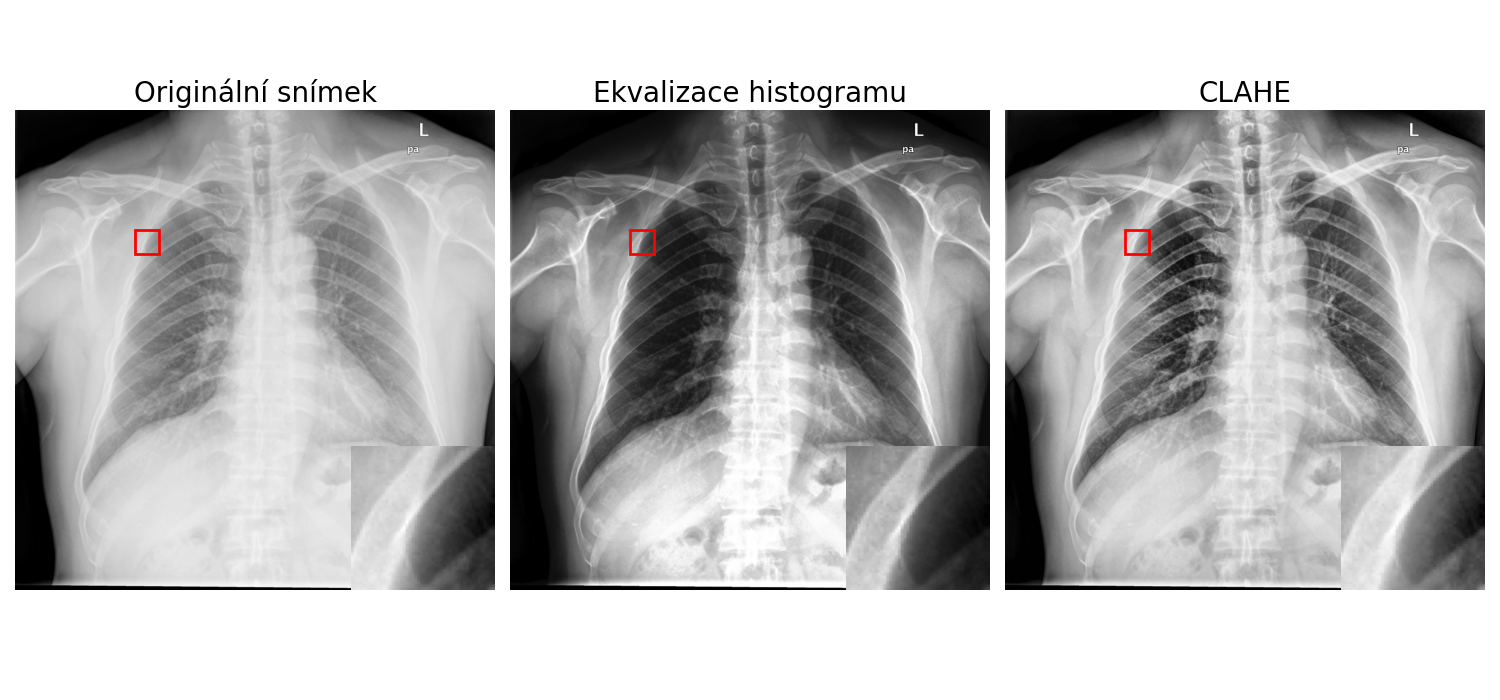
\includegraphics[width=\linewidth]{Prilohy/Obrazky/ImageEnhancement.png}
    \caption{Ukázka metod ekvalizace histogramu na rentgenovém snímku. CLAHE demonstruje lepší zachování detailů a kontrastu v porovnání s tradiční ekvalizací histogramu.}
    \label{fig:histogram_equalization}
\end{figure}

\subsubsection{Unsharp masking}
Unsharp masking je technika určená k zlepšení ostrosti obrazu tím, že zvýrazňuje hrany a detaily, které jsou v původním obrazu méně patrné. Klíčovým krokem této metody je vytvoření tzv. masky ostrých detailů, která vznikne odečtením rozmazané verze obrazu od jeho původní podoby. Rozmazaná verze obrazu se získává například pomocí Gaussova filtru, který je aplikován na původní obraz. Intenzita tohoto rozmazání určuje, jak silně budou hrany a detaily v masce zvýrazněny. Následující rovnice ukazuje získání výsledného, zaostřeného snímku pomocí techniky unsharp masking. Po získání masky ostrých detailů se tato maska přičte zpět k původnímu obrazu. Tento krok zvyšuje kontrast a ostrost obrazu, přičemž zvýrazňuje oblasti s výraznými rozdíly mezi sousedními pixely. \cite{UnsharpMasking}

\begin{algorithm}
    \caption{Unsharp Masking}
    \begin{algorithmic}[1]
        \State \textbf{Vstup:} Původní obraz $I$, standardní odchylka Gaussova filtru $\sigma$, zesílení $\lambda$
        \State \textbf{Výstup:} Vylepšený obraz $I'$
        \State $G \gets \text{Gauss}(I, \sigma)$ \Comment{Vytvoření rozmazané verze obrazu pomocí Gaussova filtru}
        \State $M \gets I - G$ \Comment{Vytvoření masky ostrých detailů odečtením rozmazaného obrazu}
        \State $I' \gets I + \lambda M$ \Comment{Zvýšení ostrosti původního obrazu přičtením masky}
    \end{algorithmic}
\end{algorithm}

V tomto procesu:
\begin{itemize}
    \item $\sigma$ určuje míru rozmazání při použití Gaussova filtru.
    \item $\lambda$ je koeficient zesílení, který kontroluje míru, jakou jsou detaily zvýrazněny při přičítání masky k původnímu obrazu.
\end{itemize}

Při použítí unsharp masking metody může vznikat nežádoucí halo efekt. Tento efekt se projevuje jako nežádoucí světelný okraj kolem kontrastních hran, což může vést k umělému a nepřirozenému vzhledu obrazu. Integrace filtru zachovávajícího hrany (edge-preserving filter) do procesu unsharp masking může být klíčová pro minimalizaci zmíněného efektu. \cite{UnsharpMasking}

Unsharp masking metoda je vhodná pro aplikace, kde je žádoucí zlepšit viditelnost detailů a hran. Důležitým aspektem při použití unsharp masking je správný výběr parametrů $\sigma$ a $\lambda$, jelikož tyto hodnoty významně ovlivňují výsledný vzhled obrazu. Příliš vysoké hodnoty mohou vést k nežádoucím artefaktům, jako jsou halo efekty kolem hran, zatímco příliš nízké hodnoty mohou mít za následek nedostatečné zvýraznění detailů.

\subsubsection{Gama korekce}
Gamma korekce je technika používaná k úpravě jasu obrazových dat. Principem této metody je aplikace nelineární transformace na původní pixelové hodnoty obrazu, čímž se upravuje celková jasová křivka podle gamma funkce. Tato korekce umožňuje efektivněji využít dynamický rozsah zobrazovacích zařízení a zlepšit viditelnost detailů v tmavých i světlých oblastech obrazu bez ztráty informací v ostatních částech obrazového spektra. \cite{PreprocessingBook}

Aplikace gamma korekce se obvykle provádí podle vzorce:
\begin{equation}
    I' = I^\gamma
\end{equation}
\begin{conditions}
    I &  původní intenzita pixelu \\
    I' & nová intenzita pixelu po aplikaci gamma korekce \\
    \gamma & gamma faktor, který určuje míru korekce
\end{conditions}

Hodnota gamma faktoru menší než 1 zvýší jas tmavších oblastí obrazu, zatímco hodnota větší než 1 ztmaví světlejší oblasti a zvýší kontrast.
 
\subsection{Redukce šumu}
Redukce šumu ve snímcích je zásadní proces v digitálním zpracování obrazu, který má za cíl odstranit nebo minimalizovat vliv šumu přidaného během akvizice nebo přenosu obrazových dat. Šum může být způsoben různými externími faktory a může výrazně snížit kvalitu a čitelnost snímků, což má negativní dopad na jejich další analýzu a interpretaci.

Šum je obvykle definován jako náhodná variace intenzity obrazových bodů (pixelů), která se projevuje jako viditelné zrnění nebo textura na snímku. Tato náhodná variabilita může být důsledkem základních fyzikálních procesů, jako je povaha fotonu světla nebo tepelná energie v senzorech obrazu. Může vzniknout v okamžiku snímání nebo při přenosu obrazu.

Jednoduchý matematický model, kterým lze vyjádřit přítomnost aditivního šumu v obrazu, můžeme definovat jako:
\begin{equation}
    f(x, y) = I(x, y) + N(x, y)
\end{equation}
\begin{conditions}
    f(x, y) & je pozorovaná intenzita pixelu se šumem \\
    I(x, y) & je skutečná intenzita pixelu bez šumu \\
    N(x, y) & je hodnota šumu přidaná k pixelu
\end{conditions}

Redukce šumu je proto klíčovým krokem ve zpracování obrazu, který pomáhá zlepšit celkovou kvalitu snímků tím, že vyhlazuje obraz a odstraňuje nepřesnosti, avšak s opatrností, aby nedošlo k ztrátě důležitých detailů nebo hran v obrazu. Efektivní algoritmy pro redukci šumu se snaží dosáhnout rovnováhy mezi odstraněním šumu a zachováním nebo dokonce zvýrazněním důležitých vlastností obrazu, jako jsou hrany nebo textury. \cite{ImageDenoisingTechniques,ImageNoiseReductionIran}

\subsubsection{Typy šumu ve snímcích}
Existuje několik typů šumu, které se mohou ve snímcích vyskytovat. Tyto šumy se liší svým původem, charakteristikami a vlivem na kvalitu obrazu. Pro účinnou redukci šumu je klíčové rozpoznat, s jakým typem šumu máme co do činění, aby bylo možné zvolit nejvhodnější metodu pro jeho odstranění. Níže jsou uvedeny některé z nejčastějších typů šumu, které mohou ovlivnit digitální snímky.

\begin{itemize}
    \item \textbf{Gaussovský šum} je pravděpodobně nejrozšířenějším typem šumu v digitálních obrazových systémech, způsobený především elektronickými fluktuacemi v senzoru a obvodech kamery. Je charakterizován normálním rozdělením intenzit pixelů kolem skutečné hodnoty s určitou střední hodnotou a standardní odchylkou. \[P(n) = \frac{1}{\sqrt{2\pi\sigma^2}} e^{-\frac{(n-\mu)^2}{2\sigma^2}}\] Gaussovský šum je obvykle považován za aditivní šum, což znamená, že jeho hodnota je nezávisle přidána k intenzitě každého pixelu. \cite{ImageDenoisingTechniques}
    \item \textbf{Impulzní šum (Šum soli a pepře)} se projevuje jako náhodné černé nebo bílé (nebo obojí) pixely rozptýlené po celém obrazu. Tento typ šumu může vzniknout kvůli chybám v senzoru nebo při přenosu dat. Na rozdíl od Gaussovského šumu je impulzní šum typicky nelineární a jeho redukce vyžaduje specifické nelineární filtrační techniky. \cite{ImageDenoisingTechniques}
    \item \textbf{Poissonův šum} je typ šumu, který je často přítomen v obrazových datech získaných z nízkých intenzit světla, jako jsou rentgenové snímky nebo mikroskopické snímky. Poissonův šum je důsledkem náhodného procesu počtu fotonů, které dopadají na senzor, a je charakterizován jako náhodný proces s diskrétním rozdělením pravděpodobnosti. Redukce Poissonova šumu vyžaduje specifické metody, které jsou schopny zacházet s diskrétními daty a zároveň zachovat důležité detaily v obraze. \cite{ImageDenoisingTechniques} Poissonův šum může být modelován jako: \[ P(n) \sim \frac{e^{-\lambda} \lambda^n}{n!}\] 
    \item \textbf{Speckle šum} se řadí do skupiny multiplikativních šumů, které jsou často přítomny v ultrazvukovém a radarovém zobrazování. Tento šum je důsledkem koherence vlnění použitého pro snímání a interferencí mezi rozptýlenými vlnami. Speckle šum může být modelován pomocí Rayleighova nebo Gamma rozdělení v závislosti na povaze obrazových dat. \cite{ImageDenoisingTechniques}
\end{itemize}

\subsubsection{Typy filtrů pro redukci šumu}
Pro efektivní redukci šumu ve snímcích jsou k dispozici různé typy filtrů, které se liší svým principem a účinností v závislosti na konkrétním typu šumu. Níže jsou uvedeny některé z nejčastěji používaných filtrů pro redukci šumu ve snímcích.

\begin{itemize}
    \item \textbf{Lineární filtrování}, také známo jako konvoluční filtrování, aplikuje lineární operátor na skupinu sousedicích pixelů v obrazu s cílem vyhladit nebo zvýraznit určité vlastnosti obrazu. Hlavní principem lineárních filtrů je konvoluce obrazu s jádrem filtru či maskou, což je malá matice daného rozměru, která určuje váhy pro každý pixel v okolí. Tyto váhy určují, jakým způsobem okolní pixely ovlivňují hodnotu pixelu výstupního obrazu. Hlavní výhodou lineárních filtrů je jejich jednoduchost a efektivita, což je dělá vhodnými pro rychlé a efektivní zpracování obrazu. Nicméně, lineární filtry mohou způsobovat neostrost hran and detailů ve snímcích. \cite{ImageDenoisingTechniques, XRayImageProcessing}
    
    \begin{equation}
        I_{filtered}(x, y) = \sum_{i=-a}^{a} \sum_{j=-b}^{b} K(i, j) \cdot I(x-i, y-j)
    \end{equation}
    \begin{conditions}
        I_{filtered}(x, y) & intenzita pixelu na pozici (x, y) ve filtrovaném snímku \\
        K(i, j) & koeficienty kernelu \\
        I(x-i, y-j) & intenzita pixelu v původním snímku v okolé pixelu (x, y) 
    \end{conditions}
    \item \textbf{Nelineární filtrování} je alternativní přístup k redukci šumu, který se zaměřuje na zachování hran a detailů v obraze. Nelineární filtry jsou schopny zacházet s nelineárními vztahy mezi pixely a jsou schopny lépe zachovat důležité strukturální vlastnosti obrazu. Nelineární filtry jsou proto obzvláště účinné při redukci impulzního či spekle šumu. \cite{ImageDenoisingTechniques, XRayImageProcessing}
\end{itemize}

\subsubsection{Gaussovský filtr}
Gaussovský filtr reprezentuje jeden z nejčastěji používaných lineárních filtrů pro redukci šumu ve snímcích. Tento filtr je založen na aplikaci Gaussova jádra na obraz, což umožňuje odstranit vysokofrekvenční šum. Gaussovský filtr je založen na principu aplikace Gaussovy funkce na vstupní obraz, která počítá vážený průměr okolí každého pixelu, s nejvyšší váhou soustředěnou na samotný pixel a se zmenšujícími se váhami pro sousední pixely na základě jejich prostorové vzdálenosti od středového pixelu. Gaussovský filtr je založen na konvoluci obrazu s Gaussovým jádrem, které je definováno jako:
\begin{equation}
    G(x, y) = \frac{1}{2\pi\sigma^2} e^{-\frac{x^2 + y^2}{2\sigma^2}}
\end{equation}
\begin{conditions}
    G(x, y) & hodnota Gaussova jádra na pozici (x, y) \\
    \sigma & standardní odchylka Gaussova jádra
\end{conditions}

Gaussovský filtr je schopen efektivně redukovat Gaussovský šum a jednou z hlavních výhod je jeho přirozená odezva na vysokofrekvenční oblasti, které potlačuje bez vytváření kroužkouvých artefaktů, které jsou běžné u low-pass filtrů.

Přestože je Gaussovský filtr velmi účinný při redukci šumu, volba směrodatné odchylky $\sigma$ je kritická. Příliš vysoká hodnota může vymazat důležité detaily spolu se šumem, zatímco příliš nízká hodnota nemusí šum dostatečně snížit. Navíc, izotropní povaha Gaussovského filtru znamená, že filtr rozmazává ve všech směrech stejnou měrou, což nemusí být žádoucí zejména tam, kde je potřeba zachování hran. \cite{XRayImageProcessing}

\begin{algorithm}
    \caption{Gaussovský filtr}
    \begin{algorithmic}[1]
        \State \textbf{Vstup:} Původní obraz $I$, standardní odchylka $\sigma$
        \State \textbf{Výstup:} Vyhlazený obraz $I_{smoothed}$
        \State Vytvořte Gaussovo jádro $G$ s rozměry $n \times n$ a $\sigma$
        \State \textbf{Inicializuj} $I_{smoothed}$ jako prázdný obraz
        \For{každý pixel $p$ v $I$}
            \State Aplikujte Gaussovo jádro na okolí pixelu $p$
            \State Nastavte hodnotu pixelu $p$ v $I_{smoothed}$ na vážený průměr hodnot v okolí
        \EndFor
        \State \textbf{return} $I_{smoothed}$
    \end{algorithmic}
\end{algorithm}

\subsubsection{Bilaterální filtr}
Bilaterální filtrování je nelineární technika pro vyhlazování obrazu, která zachovává hrany a redukuje šum. Na rozdíl od tradičních lineárních filtrů, které aplikují uniformní konvoluci napříč obrazem, bilaterální filtr kombinuje dva hlavní koncepty: prostorovou blízkost a podobnost intenzity. 

Podobně jako Gaussův filtr, bilaterální filtr používá Gaussovu funkci k vážení pixelů založeně na jejich prostorové vzdálenosti od centrálního pixelu. Tím pádem, čím jsou pixely blíže k centrálnímu pixelu, tím větší váhu mají. Unikátní pro bilaterální filtr je fakt, že váhy jsou také přizpůsobeny na základě rozdílu intenzit mezi sousedními pixely a centrálním pixelem. Pixely s podobnou intenzitou jako centrální pixel získávají vyšší váhu, což umožňuje zachování ostrých hran a detailů. Pro každý pixel ve zpracovávaném obrazu filtr vyhodnotí jeho sousedy a aplikuje váhy založené na dvou zmíněných kritériích.\cite{BilateralFilter}

Matematický vzorec pro bilaterální filtr aplikovaný na pixel p v obrazu I lze vyjádřit jako:
\begin{equation}
    BF[I](p) = \frac{1}{W_p} \sum_{q \in S} G_{\sigma_s}(||p-q||) \cdot G_{\sigma_r}(|I_p - I_q|) \cdot I_q
\end{equation}
\begin{conditions}
    BF[I](p) & hodnota pixelu po aplikaci bilaterálního filtru \\
    W_p & je normalizační faktor zajišťující, že součet vah je roven jedné \\
    G_{\sigma_s} & prostorová Gaussova funkce, která snižuje vliv vzdálených pixelů na základě prostorové vzdálenosti ||p-q|| se standardní odchylkou $\sigma_s$ \\
    G_{\sigma_r} & rozsahová Gaussova funkce, která redukuje vliv pixelů q na základě rozdílu intenzit $|I_p-I_q|$ se standardní odchylkou $\sigma_r$ \\
    I_p & hodnota pixelu p \\
    I_q & hodnota pixelu q \\
\end{conditions}

\begin{equation}
    W_p = \sum_{q \in S} G_{\sigma_s}(||p-q||) \cdot G_{\sigma_r}(|I_p - I_q|)
\end{equation}

Na rozdíl od Gaussova filtru, který aplikuje vyhlazování uniformně a může vést k rozmazání ostrých hran, bilaterální filtr nabízí sofistikovanější přístup k redukci šumu. Jeho schopnost zachovat ostré hrany při současném snížení šumu v homogenních oblastech obrazu činí bilaterální filtr vysoce ceněným nástrojem v pokročilém zpracování obrazu. Avšak, s touto schopností přichází zvýšená výpočetní náročnost a potřeba pečlivého nastavení parametrů $\sigma_s$ a $\sigma_r$, což jsou aspekty, které je třeba zvážit pro dosažení optimálních výsledků. \cite{BilateralFilter}

\subsubsection{Wienerův filtr}
Wienerův filtr je adaptivní lineární filtr, který je často používán pro redukci aditivního šumu ve snímcích s cílem zachovat důležité detaily a strukturální vlastnosti obrazu. Wienerův filtr funguje na principu minimalizace střední kvadratické chyby (anglicky minimum mean squared error - MMSE)\footnote{MSE je metrika, která měří rozdíl mezi odhadovanými a skutečnými hodnotami. V případě Wienerova filtru se minimalizuje rozdíl mezi původním obrazem a obrazem se šumem.} mezi původním obrazem a obrazem se šumem. Matematicky je Wienerův filtr navržen tak, aby našel spektrální rovnováhu mezi inverzním filtrováním signálu a vyhlazováním šumu, s ohledem na výkonová spektra signálu a šumu. Odezva filtru je vypočítána pomocí výkonových spekter, což vede k optimálnímu vyvážení mezi inverzním filtrováním pro obnovu obrazu a potlačením šumu.

\begin{equation}
    G(u,v) = \frac{1}{H(u,v)} \left[ \frac{\left| H(u,v) \right|^2}{\left| H(u,v) \right|^2 + \frac{S_{\eta}}{S_f}} \right]
\end{equation}
\begin{conditions}
    G(u,v) & odhad originálního obrazu \\
    H(u,v) & degradační funkce \\
    S_{\eta} & výkonové spektrum šumu \\
    S_f & výkonové spektrum originálního obrazu
\end{conditions}

Tento vztah představuje schopnost Wienerova filtru vyvažovat mezi inverzním filtrováním a vyhlazováním šumu s ohledem na degradační funkci a poměr signálu a šumu $\frac{S_{\eta}}{S_f}$\footnote{Poměr signálu a šumu (SNR) udává poměr mezi obrazem a úrovní šumu v daném obraze. Vysoká hodnota SNR značí, že signál je silnější než šum, což znamená, že obraz má vysokou kvalitu s minimálním množstvím šumu. Naopak nízká hodnota SNR indikuje, že šum je dominantní a signál je obtížně rozeznatelný.}. Filtr je více nakloněn k inverznímu filtrování, kde je magnituda degradační funkce velká vzhledem k šumu (vysoké SNR), a více k vyhlazování v opačném případě. \cite{WienerFilters}

\subsubsection{Mediánový filtr}
Medianový filtr je robustní nelineární filtrační technika, který se používá k redukci impulzního šumu (šumu soli a pepře). Medianový filtr funguje tak, že posouvá okno po každém pixelu obrazu, shromažďuje hodnoty pixelů z okolí daného pixelu a nahrazuje středový pixel mediánem těchto hodnot. Okno, které se obvykle používá, je čtvercové (např. 3x3, 5x5) v závislosti na stupni šumu a požadované úrovni zachování detailů. Na rozdíl od průměrových filtrů, které také snižují šum, ale mají tendenci rozmazávat hrany, medianový filtr hrany zachovává. Dále také medianový filtr nezávisí na předpokladu, že šum je specifického typu nebo variance.

\begin{algorithm}
    \caption{Medianový filtr}
    \begin{algorithmic}[1]
        \State \textbf{Vstup:} Původní obraz $I$, velikost okna $k$
        \State \textbf{Výstup:} Obraz po redukci šumu $I_{filtered}$
        \State \textbf{Inicializuj} $I_{filtered}$ jako prázdný obraz
        \For{každý pixel $p$ v $I$}
            \State \text{okolí} $\gets$ \text{extrahuj\_okolí}($I$, $p$, $k$)
            \State \text{medián} $\gets$ \text{vypočti\_medián}(okolí)
            \State \text{Nastavte hodnotu pixelu} $p$ v $I_{filtered}$ na \text{medián}
        \EndFor
        \State \textbf{return} $I_{filtered}$
    \end{algorithmic}
\end{algorithm}

Přestože je medianový filtr účinný, má svá omezení, zejména při vysokých úrovních šumu nebo když mají obrazy jemné strukturální detaily. Za těchto podmínek může filtr odstranit užitečné informace spolu se šumem. Navíc jeho výkon se může zhoršit, pokud není velikost okna správně zvolena, protože příliš velké okno může odstranit příliš mnoho detailů, zatímco příliš malé okno nemusí efektivně odstranit dostatek šumu.

\subsubsection{Filtr ne-lokálních průměrů}
Filtr ne-lokálních průměrů, anglicky Non-Local Means (NLM), představuje pokročilou techniku pro odstranění šumu z obrazu (převážně gaussovského šumu), která se vyznačuje výrazným zachováním detailů a hran. Na rozdíl od tradičních metod, které pracují s lokálními okolími pixelů, NLM vyhledává podobné fragmenty (patche) po celém obrazu a využívá jejich informace pro inteligentní vyhlazení cílového pixelu nebo oblasti, čímž se minimalizuje ztráta důležitých vizuálních prvků. NLM můžeme rozdělit na dvě varianty: pixelwise a patchwise NLM.

První varianta, pixelwise NLM, se zaměřuje na každý pixel individuálně. Pro každý pixel p ve vstupním obraze 
I se vypočítává jeho nová hodnota jako vážený průměr hodnot všech pixelů v obraze. Váhy závisí na podobnosti malých okolí (patchů) okolo každého pixelu a jsou určeny Euklidovskou vzdáleností mezi hodnotami pixelů v těchto okolích. Matematicky lze pixelwise NLM vyjádřit pomocí vztahu:

\begin{equation}
    I_{new}(p) = \frac{\sum_{q \in I} w(p,q) \cdot I(q)}{\sum_{q \in I} w(p,q)}
\end{equation}
\begin{conditions}
    w(p,q) & představuje váhu založenou na podobnosti mezi okolím pixelů p a q \\
    I(q) & hodnota pixelu q ve vstupním obraze
\end{conditions}

Druhá varianta, patchwise NLM, rozšiřuje přístup pixelwise metody tím, že jako základní jednotku pro výpočet váženého průměru bere celé patche namísto jednotlivých pixelů. Tím se zvyšuje robustnost metody vůči šumu, jelikož se lépe využívá strukturální informace z obrazu. Vztah pro patchwise NLM může být zapsán obdobně, avšak s důrazem na porovnávání celých patchů.

Rozdíl mezi pixelwise a patchwise variantami spočívá v měřítku, na kterém se hodnotí podobnost mezi částmi obrazu. Zatímco pixelwise varianta se soustředí na detailní porovnání na úrovni pixelů, patchwise přístup poskytuje robustnější odhad tím, že zapojuje větší kontext okolí zkoumaného bodu.

Algoritmus NLM, ať už v pixelwise či patchwise variantě, nabízí vynikající schopnost odstraňování šumu při zachování ostrých hran a detailů. Jeho hlavní nevýhodou však zůstává vysoká výpočetní náročnost, zejména v důsledku nutnosti porovnávat velké množství oblastí napříč celým obrazem. To činí aplikaci NLM, především v reálném čase, výzvou. Optimalizace a využití paralelního zpracování však mohou tuto nevýhodu zmírnit. \cite{NonLocalMeans}

\subsubsection{Lokálně adaptivní mediánový filtr}
Lokálně adaptivní mediánový filtr je inovativní metodou redukce šumu, specificky navrženou pro typ šumu speckle. Tento typ šumu je výsledkem interferencí mezi koherentními vlnami odraženými od cíle, což vede k zrnitému vzoru v pořízeném obraze. Tento filtr využívá lokální statistiky pro detekci speckle šumu a jeho nahrazení mediánovou hodnotou z lokálního okolí.

Nejdříve je nutné zjistit celkový součet intenzit pixelů v určitém oblastním okně, které obklopuje centrální pixel. Tento součet je základem pro další výpočty statistik, jako je lokální průměr.
\begin{equation}
    S(i, j) = \sum_{n=j-k}^{j+k}\sum_{m=i-k}^{i+k} d(m, n)
\end{equation}
\begin{conditions}
    k & poloměr posuvného okna okolo středového pixelu \\
    d(m, n) & hodnota pixelu na pozici (m, n)
\end{conditions}

Dále se určí průměrná hodnota a lokální standardní odchylka hodnot pixelů v posuvném okně. Lokální průměr pomáhá rozlišit oblasti s vysokým a nízkým šumem tím, že poskytuje základní hodnotu pro porovnání s ostatními pixely. Standardní odchylka je míra variability nebo rozptylu hodnot pixelů kolem lokálního průměru, která pomáhá identifikovat pixely s výrazně odlišnými intenzitami (tj. šum).
\begin{equation}
    \mu(i, j) = \frac{S(i, j)}{N(i, j)}
\end{equation}
\begin{conditions}
    S(i, j) & součet všech hodnot pixelů v posuvném okně \\
    N(i, j) = (2k + 1)^2 & počet pixelů v posuvném okně
\end{conditions}

\begin{equation}
    \sigma(i, j) = \sqrt{\frac{\sum_{m=i-k}^{i+k} \sum_{n=j-k}^{j+k} (d(m, n) - \mu(i, j))^2}{N(i, j)}}
\end{equation}
\begin{conditions}
    \mu(i, j) & lokální průměr hodnot pixelů v posuvném okně
\end{conditions}

Na základě definováné dolní a horní hranice pro rozpoznání validních pixelů v rámci posuvného okna se rozhodne, které pixely jsou považovány za validní, a které představují potenciální šum.
\begin{equation}
    \begin{split}
        LB(i, j) &= \mu(i, j) - M \cdot \sigma(i, j) \\
        UB(i, j) &= \mu(i, j) + M \cdot \sigma(i, j)
    \end{split}
\end{equation}
\begin{conditions}
    \mu(i, j) & lokální průměr hodnot pixelů v posuvném okně \\
    \sigma(i, j) & lokální standardní odchylka hodnot pixelů v posuvném okně \\
    M & uživatelem definovaný násobitel pro určení prahu šumu
\end{conditions}

\begin{equation}
    l(m, n) = 
    \begin{cases} 
        0 & \text{pokud } d(m, n) < LB(i, j) \text{ nebo } d(m, n) > UB(i, j) \\
        1 & \text{pokud } LB(i, j) \leq d(m, n) \leq UB(i, j)
    \end{cases}
\end{equation}
\begin{conditions}
    LB(i, j), \ UB(i, j) & dolní a horní hranice pro validní hodnoty pixelů
\end{conditions}

Finální rovnice nahrazuje hodnotu centrálního pixelu, identifikovaného jako šum, mediánovou hodnotou z validních pixelů v okně. Tento proces zajišťuje, že hodnota pixelu reprezentuje jeho skutečné okolí a zlepšuje tak celkovou kvalitu obrazu redukcí šumu.
\begin{equation}
    r(i, j) = \text{median } d(m, n) \text{ | } l(m, n) = 1, i-k \le m, n \le i+k
\end{equation}
\begin{conditions}
    l(m, n) & maska určující, zda je pixel na pozici $(m, n)$ považován za validní nebo za šum
\end{conditions}

Lokálně adaptivní mediánový filtr se ukazuje jako výrazně efektivní při odstraňování speckle šumu, což je běžný problém v rentgenových a jiných druzích medicínských snímků. Využití lokálních statistik umožňuje filtru selektivně cílit na šumové pixely, zatímco zachovává ostré hrany a důležité detaily, což je klíčové pro zachování diagnostické hodnoty obrazu.

Nicméně, stejně jako většina pokročilých metod zpracování obrazu, i tento filtr má své nevýhody. Především je to jeho výpočetní náročnost, která může být limitující pro aplikace v reálném čase nebo při zpracování velkých datasetů. Navíc, efektivní využití filtru vyžaduje pečlivý výběr parametrů, což může vyžadovat pokročilé znalosti a experimentální ladění pro dosažení optimálních výsledků. \cite{LocalAdaptiveMedianFilter}

\begin{figure}[ht]
    \centering
    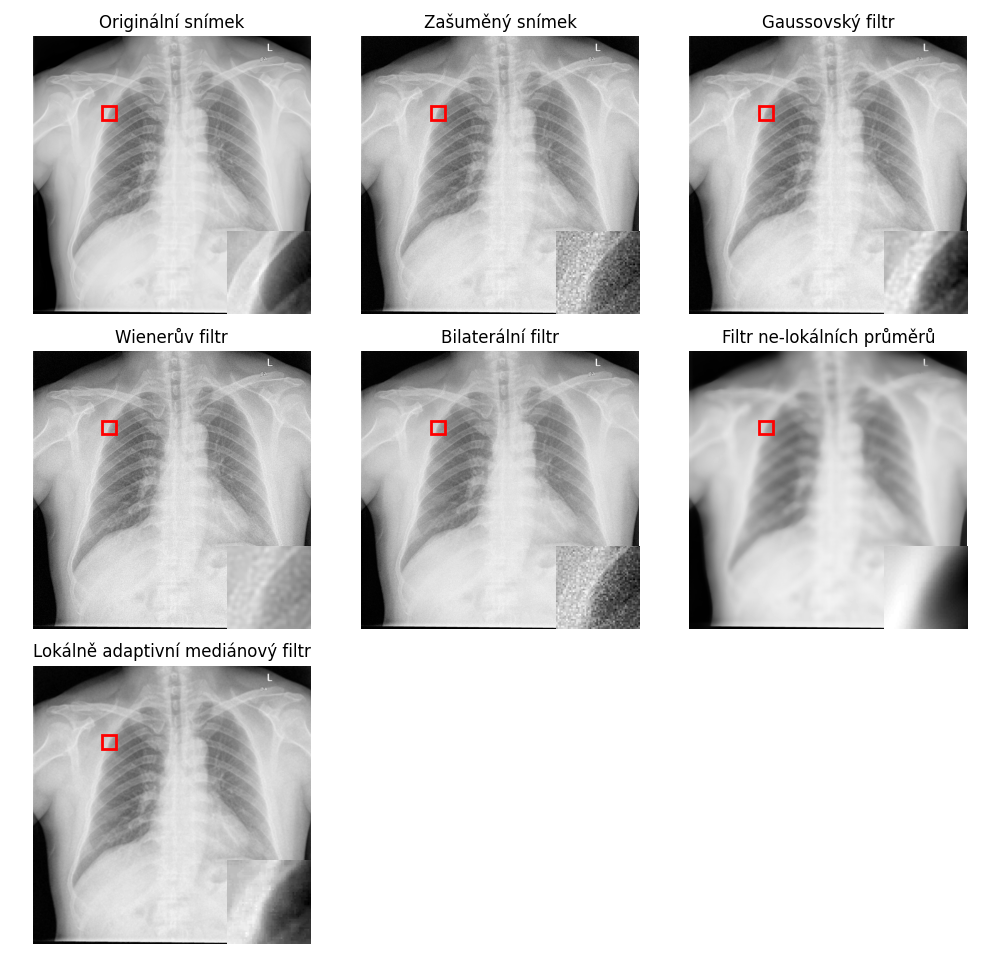
\includegraphics[width=\linewidth]{Prilohy/Obrazky/NoiseReduction.png}
    \caption{Snímky demonstrují účinky popsaných filtrů na kvalitu obrazu v porovnání s originálním snímkem a snímkem po umělém přidání šumu, aby se simulovalo běžné zkreslení vznikající během akvizice obrazu.}
    \label{fig:noise_reduction_filters}
\end{figure}

% \subsection{Prahování a binarizace} TODO: if not enough pages write this as well

\section{Neuronové sítě pro předzpracování obrazu}
Předchozí sekce byla věnována klasickým metodám předzpracování obrazu, kde byl brán důraz na techniky pro vylepšení obrazu a odstranění či redukci různých typů šumu ze snímků. Tato sekce se bude zabývat pokročilým oborem pro předzpracování obrazu, kterým jsou neuronové sítě.

Neuronové sítě představují významný skok v možnostech zpracování obrazu, především díky jejich schopnosti učit se a generalizovat na základě velkých datových sad. Na rozdíl od klasických metod, které aplikují pevně stanovená pravidla, se neuronové sítě dokáží přizpůsobit na základě konkrétních charakteristik a variací v datech, na kterých jsou trénovány. Tato adaptabilita je klíčová pro zpracování obrazů v dynamických a různorodých podmínkách, což zahrnuje vše od standardního zlepšování obrazu po složité úlohy jako je rozpoznávání objektů nebo segmentace obrazu.

Neuronové sítě, a zvláště konvoluční neuronové sítě (CNN), jsou vysoce efektivní v automatickém učení a rozpoznávání vzorců z obrazových dat. Tyto sítě simulují způsob, jakým lidský mozek zpracovává vizuální informace, což umožňuje extrakci a učení vysokého řádu charakteristik, které jsou následně využity pro klasifikaci nebo predikci. Díky této schopnosti se neuronové sítě stávají základem mnoha pokročilých systémů pro automatizované zpracování obrazu.

Využití neuronových sítí však také přináší výzvy, včetně potřeby velkého množství anotovaných trénovacích dat a výpočetně náročných modelů, které mohou vyžadovat specializovanou hardwarovou podporu pro efektivní trénink a nasazení. 

Následující sekce bude zaměřena na nejčastěji využívané architekty neuronových sítí pro předzpracování obrazu, s důrazem na konvoluční neuronové sítě (CNN). \cite{CNNConcepts}

\subsection{Úvod do konvolučních neuronových sítí}
Neuronové sítě jsou základním stavebním prvkem moderního strojového učení a mají zásadní význam pro rozvoj oblastí jako je zpracování přirozeného jazyka či obrazu, rozpoznávání objektů v obraze, při analýze signálu, v robotice a mnoha jiných důležitých oborech. Tyto systémy jsou inspirovány strukturou a funkcí lidského mozku a jsou navrženy tak, aby modelovaly složité vzory a vztahy v datech. Strukturálně jsou neuronové sítě složeny z vrstev neuronů, což jsou jednotky zpracovávající informace, které jsou propojeny spojeními, ohodnocenými vahami.

\subsubsection{Hlavní komponenty neuronových sítí}
Základem neuronové sítě je její architektura, která je definována několika klíčovými komponentami. Tyto komponenty jsou základem pro učení a zpracování dat v síti. V následujícím seznamu jsou jednotlivé komponenty podrobněji popsány:

\begin{itemize}
    \item \textbf{Neuron} Neuron v neuronové síti je elementární jednotka, která simuluje chování neuronu v biologických systémech. Přijímá vstup $x = (x_1, x_2, x_3, ..., x_n)$, který je zpracován a následně vrácen na výstupu. Tento výstup je vstupen do dalšího neuronu nebo je součástí koncového výstupu ze sítě.
        \begin{equation}
            z = W \cdot x + b
        \end{equation}
        \begin{conditions}
            W & reprezentuje váhy, jenž jsou parametry určující sílu signálu mezi neurony. \\
            b & bias, což je parametr posunutí, který upravuje výstup neuronu před aplikací aktivační funkce.
        \end{conditions}
    \item \textbf{Vrstvy (Layers)} Vrstvy se skládají z neuronů a jsou základem architektury neuronové sítě. Každá vrstva plní specifickou funkci v procesu učení. Vrstvy mohou být kategorizovány do tří typů:
        \begin{itemize}
            \item \textbf{Vstupní vrstva (Input layer)} Tato vrstva přijímá surová data a připravuje je pro další zpracování v síti. Každý neuron této vrstvy přímo reprezentuje jednu vlastnost vstupního datového vektoru.
            \item \textbf{Skyté vrstvy (Hidden layers)} Skryté vrstvy jsou mezi vstupní a výstupní vrstvou a jejich úkolem je zpracování signálů přijatých od vstupní vrstvy. Komplexnost a hloubka těchto vrstev jsou klíčové pro schopnost sítě učit se složité vzory.
            \item \textbf{Výstupní vrsta (Output layer) } Poslední výstupní vrstva generuje predikce určené neuronovou sítí. Například v klasifikačních úlohách může tato vrstva používat softmax funkci\footnote{Softmax funkce se často používá jako aktivační funkce v poslední vrstvě neuronové sítě při klasifikačních úlohách. Tato funkce převádí výstupní hodnoty neuronů na pravděpodobnostní rozdělení mezi různými třídami. Matematický vzorec pro softmax funkci je definován následovně: $\text{softmax}(z_i) = \frac{e^{z_i}}{\sum_{j=1}^{N} e^{z_j}}$}.
        \end{itemize}
    \item \textbf{Aktivační funkce (Activation function)} Aktivační funkce je důležitou složkou neuronových sítí, která umožňuje modelování nelineárních vztahů. Funkce, jako je sigmoid, tanh a ReLU (Rectified Linear Unit), jsou běžně používány k výpočtu výstupu z neuronů na základě vstupu a vah. Například, ReLU, která je definována jako $ReLU(x) = max(0, x)$, je populární pro svou schopnost rychle konvergovat během tréninku a minimalizovat problém mizejících gradientů\footnote{Mizející gradienty jsou problém, kdy gradient ztrátové funkce klesá exponenciálně rychle s každou vrstvou v síti, což způsobuje, že váhy v raných vrstvách se téměř neaktualizují. Tento jev výrazně zpomaluje trénink a může způsobit, že síť nedokáže efektivně učit složité vzory.}.
    \item \textbf{Ztrátová funkce (Loss function)} Ztrátová funkce, někdy nazývaná penalizační funkce, poskytuje kvantitativní hodnocení toho, jak daleko jsou predikce neuronové sítě od skutečných hodnot. Během tréninku neuronové sítě je hlavním cílem minimalizace této funkce. Mezi běžné ztrátové funkce se řadí střední kvadratická chyba (MSE) pro regresní úkoly a cross-entropy pro klasifikační úkoly. 
    \item \textbf{Optimalizační algoritmus (Optimizer)} Optimalizační algoritmy jsou základem učení neuronových sítí, protože určují, jak se síť učí z dat tím, že iterativně upravují váhy a biasy k minimalizaci ztrátové funkce. Stochastic Gradient Descent (SGD) provádí tuto úpravu tak, že v každém kroku tréninku náhodně vybere vzorek dat a spočítá gradient ztrátové funkce pouze na základě tohoto vzorku:
    Adam a RMSprop jsou pokročilejší varianty, které se snaží zlepšit konvergenci SGD tím, že upravují rychlost učení pro každý parametr individuálně, což může vést k rychlejšímu a stabilnějšímu učení, zejména v komplexních sítích.
\end{itemize}

\begin{figure}[ht]
    \centering
    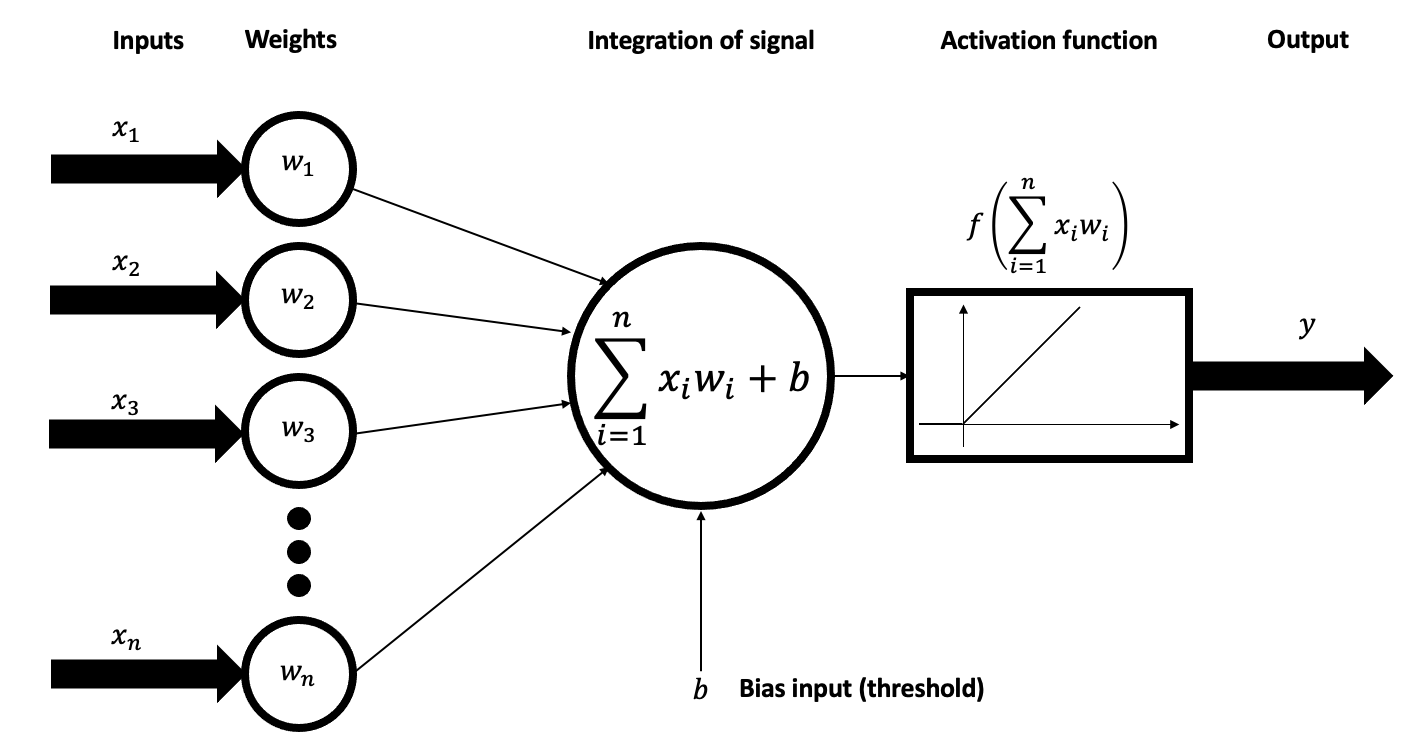
\includegraphics[width=\linewidth]{Prilohy/Obrazky/NNComponents.png}
    \caption{Ilustrace neuronové jednotky, ukazující základní komponenty jako vstup, váhy, bias, aktivační funkci a výstup. (převzato z \cite{NNComponentsIMG} pod licencí CC BY-SA 4.0)}
    \label{fig:nn_components}
\end{figure}

Základní komponenty neuronových sítí hrají zásadní roli ve funkcionalitě vytvořených modelů. Neurony a vrstvy formují strukturu sítě, zatímco aktivační funkce umožňují modelování nelineárních vztahů, což je nezbytné pro zpracování složitých vzorů a funkcí. Ztrátové funkce poskytují metriku pro hodnocení úspěšnosti sítě v předpovídání a jsou klíčové pro navigaci procesu učení. Optimalizační algoritmy řídí tento učící se proces tím, že iterativně upravují interní parametry sítě, aby se minimalizovala celková ztráta a zvýšila přesnost modelu. Každá z těchto komponent společně zajišťuje, že neuronové sítě se mohou učit efektivně, adaptovat se a poskytovat přesné predikce při řešení zadaných úloh. \cite{CNNConcepts, CNNConcepts2}

\subsubsection{Základy konvolučního zpracování v CNN}
Jak již bylo zmíněno výše, konvoluční neuronové sítě (CNN) jsou specializovaným druhem neuronových sítí, které se používají především pro zpracování strukturovaných dat, jako jsou například obrazová data. CNN jsou známé svou schopností zachytit prostorové a časové závislosti v obraze pomocí aplikace příslušných filtrů. Úloha konvolučních operací je jádrem toho, co činí CNN tak efektivními pro úlohy, jako je rozpoznávání obrazu, klasifikace obrazu a detekce objektů.

Operace konvoluce zahrnuje posunutí jádra (kernelu) přes vstupní data (obvykle obraz) a výpočet skalárního součinu jádra s překrývajícími se části obrazu. Výsledek tvoří jednu položku ve výstupní mapě příznaků. Tento proces se opakuje posouváním jádra po všech pozicích vstupní matice. Mezi klíčové aspekty konvoluce patří:

\begin{itemize}
    \item \textbf{Jádro konvoluce} Malé matice používané k detekci specifických prvků, jako jsou hrany nebo textury ve vstupním obraze. Každý filtr je navržen tak, aby zachytil určitý aspekt vstupních dat.
    \item \textbf{Krok jádra} Počet pixelů, o které posouváme filtr po vstupním obraze. To ovlivňuje velikost výstupní mapy prvků.
    \item \textbf{Padding} Existuje několik možností, jak umožnit jádru brát v potaz i hraniční prvky. Jednou z možnosti je přidání vrstev nul kolem vstupního obrazu. Další možností je použití zrcadlení (mirror padding), kde se okrajové prvky zrcadlově opakují, což pomáhá jádru zahrnout informace z okrajů obrazu bez ztráty dat.
    \item \textbf{Mapa příznaků} Výstup operace konvoluce se nazývá mapa příznaků. Představuje odezvu filtru v každé prostorové poloze. Použitím různých filtrů může síť CNN zachytit širokou škálu aspektů vstupního obrazu.
\end{itemize}

Dalším důležitým konceptem v CNN je poolování, které se obvykle používá po operaci konvoluce. Nejběžnější formou sdružování je tzv. max pooling, kdy výstupem sdružovacího jádra je maximální hodnota z části mapy, kterou pokrývá. Tato operace snižuje dimenzionalitu mapy příznaků a umožňuje síti být odolnou vůči malým změnám vstupního obrazu.

V hlubokých konvolučních neuronových sítích se vrství několik konvolučních a sdružovacích vrstev za sebou, což síti umožňuje učit se hierarchické rysy. Nižší vrstvy se mohou naučit rozpoznávat jednoduché rysy, jako jsou hrany, zatímco hlubší vrstvy mohou interpretovat složité aspekty, jako jsou objekty.

Konvoluce je základní operací v CNN, která umožňuje extrakci smysluplných rysů ze vstupních dat. Díky vrstvení a kombinaci konvolučních, aktivačních a sdružovacích vrstev se CNN mohou efektivně naučit hierarchii rysů, která je klíčová pro zvládání složitých úloh vizuálního rozpoznávání. Každá složka, od výběru filtrů až po použití poolingu, hraje rozhodující roli při definování schopnosti sítě přesně interpretovat a klasifikovat vstupní data. \cite{CNNConcepts, CNNConcepts2}

\subsection{Autoenkodéry v oblasti zpracování obrazu}
Autoenkodéry jsou samostatnou třídou modelů neuronových sítí určených především k učení efektivního kódování dat. Tyto sítě toho dosahují komprimací vstupu do méně rozměrné reprezentace latentního prostoru a následnou rekonstrukcí výstupu z této komprimované podoby. Tento duální proces kódování a následného dekódování neslouží pouze ke kompresi dat, ale má zásadní význam pro to, aby síť byla nucena upřednostňovat a zachycovat nejvíce informativní rysy dat.

\subsubsection{Struktura autoenkodérů}
Autoenkodéry se dělí na tři hlavní části:

\begin{itemize}
    \item \textbf{Enkodér} Proces kódování zahrnuje transformaci vstupních dat s vysokou dimenzí do komprimované podoby. Tento krok je klíčový, protože umožňuje modelu naučit se podstatu dat odfiltrováním šumu a redundance. Tím se síť naučí reprezentaci, která zachycuje základní vzory a struktury nezbytné pro rekonstrukci vstupních dat. Enkodér přebírá vstupní vektor $x$ a převede jej na komprimovanou reprezentaci $z$, často označovaný jako latentní prostor:
    \begin{equation}
        z = \sigma(W_e \cdot x + b_e)
    \end{equation}
    \begin{conditions}
        W_e & matice vah enkodéru. \\
        b_e & bias vektor enkodéru. \\
        \sigma & nelineární aktivační funkce.
    \end{conditions}
    \item \textbf{Latentní prostor (bottleneck)} Srdcem autoenkodéru je jeho latentní prostor, v němž jsou vstupní data reprezentována ve své nejkomprimovanější podobě. Tato reprezentace poskytuje pohled na data v nižší dimenzi a zdůrazňuje jejich nejdůležitější atributy. Rozměrnost a konfigurace latentního prostoru jsou velmi důležité a ovlivňují, jak efektivně dokáže autokodér komprimovat a rekonstruovat data.
    \item \textbf{Dekodér} Proces dekódování se snaží co nejpřesněji rekonstruovat původní vstup z komprimované zakódované reprezentace. V této fázi se testuje kvalita naučených rysů a účinnost kódování. Cílem není dosáhnout dokonalé rekonstrukce, ale spíše vytvořit aproximaci, která zachová nejvýznamnější atributy původních dat. Tato schopnost je užitečná zejména v aplikacích, kde je pochopení základní struktury dat cennější než reprodukce přesné kopie. Dekódovací část rekonstruuje vstupní data $x'$ z latentní reprezentace $z$.
\end{itemize}

Autoenkodéry se používají v celé řadě aplikací, které přesahují rámec prosté komprese dat. Například při redukci šumu se naučí ignorovat náhodné odchylky ve vstupních datech a místo toho se soustředí na rekonstrukci smysluplného základního vzoru obrazu. Používají se také při detekci anomálií, kdy se naučí dobře reprodukovat typické případy dat, ale mají problémy s reprodukcí odlehlých hodnot, a tím identifikují anomální data. V oblasti zpracování obrazu se autoenkodéry také využívají pro segmentaci obrazu a extrakci rysů. Tyto schopnosti jsou klíčové pro rozpoznávání objektů a detailní analýzu obrazového obsahu. \cite{Autoencoders, AutoencodersIntroduction}

\section{Obecné postupy augmentace dat}
Augmentace dat neboli rozšiřování dat je klíčovou technikou v oblasti strojového učení, zejména v oblastech zpracování obrazu a počítačového vidění. Zahrnuje umělé rozšíření velikosti a rozmanitosti datové sady použitím řady transformací, které jsou aplikovány na vstupní data. Tato sekce se bude zabývat konceptem augmentace dat, důvody použití se zdůrazněním na přínos i omezení při aplikace augmentace a v neposlední řadě budou popsány jedny z nejpoužívanějších technik rozšiřování dat.

\subsection{Augmentace dat}
Augmentace dat je mocný nástroj používaný ve strojovém učení ke zvětšení velikosti a rozmanitosti datových sad, což je zvláště výhodné při trénování modelů hlubokého učení. Podstata augmentace dat spočívá v aplikaci řady deterministických nebo náhodných transformací na trénovací vzorky s cílem vytvořit nová, rozmanitá data. Tento proces pomáhá simulovat variabilitu, s níž se model může setkat v reálných scénářích, a tím zlepšuje jeho zobecňovací schopnosti.

Rozšířování dat zahrnuje několik kroků a technik, z nichž každá má za cíl upravit původní data tak, aby odrážela možné odchylky v reálném světě, aniž by se změnilo vlastní označení nebo význam dat. V případě obrázků to mohou být geometrické transformace, rozšíření barevného prostoru, jádrové filtry nebo zamíchání obrázků. Rozšířená data jsou pak vložena do procesu trénování spolu s původními daty. Takto rozšířená sada dat poskytuje modelu ucelenější sadu příkladů, z nichž se může učit, a pokrývá tak širší škálu variant, než jakou by mohla nabídnout samotná původní sada dat. Augmentace dat může být iterativní proces, při kterém se v různých trénovacích epochách používají různé kombinace transformací. Toto neustálé zavádění variací může zabránit tomu, aby se modely příliš zaměřovaly na konkrétní variace trénovacích dat a tím se zabraňovalo možnému přeučený trénovaného modelu\footnote{Přeučení, nebo "overfitting", je jev, kdy model strojového učení příliš přesně odpovídá omezené sadě trénovacích dat, což způsobuje, že má potíže s generalizací na nová, neviděná data.}. \cite{AugmentationBasics, AugmentationSurvey}

\subsection{Přínos a omezení při rozšiřování dat}
Rozšířování dat může být dvousečná zbraň při využití ve strojovém učení, zejména v úlohách zahrnujících složité typy dat, jako jsou obrázky. Může sice významně zvýšit schopnost modelu schopnost zobecňovat na základě trénovacích dat, ale pokud není výběr augmentačních metod promyšlený, představuje také riziko. Tato podsekce se zabývá výhodami a omezeními rozšiřování dat a zdůrazňuje důležitost výběru vhodných strategií rozšiřování pro konkrétní úlohy.

\subsubsection{Benefity rozšiřování dat}
Zavedení realistických variací do trénovacích dat umožňuje modelům lépe se přizpůsobit a efektivně fungovat v široké škále scénářů, které mohou přesahovat podmínky zastoupené v původní datové sadě. Tato schopnost je nezbytná zejména v oblastech, kde je obtížné nebo finančně náročné získat rozmanité a rozsáhlé datové sady. Například ve zdravotnictví nebo v autonomních vozidlech, kde musí modely rozpoznávat a reagovat na nečekané situace, které nebyly přímo součástí trénovacích dat. Augmentace dat také zvyšuje efektivní velikost datové sady, což je klíčové pro minimalizaci přeučení modelu. Tím, že model není vystaven pouze omezenému počtu vzorů, se snižuje riziko, že by se model příliš zaměřil na irelevantní detaily, které nejsou užitečné pro generalizaci na nová data. Dále techniky jako vnášení šumu, ořezávání a rotace přispívají k zvýšení odolnosti modelu vůči různým změnám a zkreslením vstupů, což je kritické pro aplikace v reálném světě, kde jsou vstupní data často nepředvídatelná a různorodá. \cite{AugmentationBasics, AugmentationSurvey}

\subsubsection{Omezení rozšiřování dat}
Přestože augmentace dat nabízí řadu výhod, je důležité přistupovat k jejímu využití opatrně. Nevhodně zvolené metody rozšiřování dat mohou vést k zavádějícím nebo irelevantním změnám ve vstupních datech, což může způsobit, že se modely naučí nesprávné vzorce a budou generovat chybné predikce na nových datech. Kromě předchozích popsaných omezení může zvětšení datové sady vést ke zvýšení výpočetní náročnosti, zejména ve fázích trénování modelů. Složité transformace a generování velkého objemu augmentovaných dat vyžadují výkonnější hardware a delší trénovací časy, což může být v některých situacích nepraktické nebo finančně náročné.

Například v projektu zaměřeném na detekci a klasifikaci vozidel v městské dopravě pomocí hlubokého učení byl učiněn pokus o zvětšení souboru dat použitím náhodného škálování snímků. Záměrem bylo zajistit, aby byl model odolný vůči změnám velikosti vozidla v důsledku vzdálenosti od kamery. Zvolený faktor škálování byl však příliš agresivní, neboť některá vozidla byla zmenšena na velikost, která neodpovídá reálným scénářům nebo byla zvětšena tak, že se nerealisticky překrývala s jinými objekty nebo hranicemi scény. Tato nesprávná aplikace vedla k několika problémům:

\begin{itemize}
    \item \textbf{Zmatení modelu} Model začal špatně klasifikovat malá vozidla, jako jsou motocykly či kola ale také příliš velká vozidla, jako jsou autobusy nebo nákladní vozidla, protože měřítko těchto vozidel v augmentovaných obrázcích nesouhlasilo s typickými měřítky pozorovanými v reálných dopravních podmínkách. 
    \item \textbf{Prostorová nekonzistence} Přehnané měřítko narušilo prostorové vztahy a proporce ve scéně, které jsou klíčové pro kontextové porozumění v úlohách detekce objektů.
    \item \textbf{Neefektivnost tréninku} Model měl problémy během tréninku konvergovat, protože nadměrná variabilita ve velikostech objektů zavedená augmentací vedla k odchýlení při učení správných rysů, které definují různé typy vozidel ve standardních měřítcích. 
\end{itemize}

Tento příklad zdůrazňuje důležitost aplikace transformací, které odrážejí realistické variace. Augmentace dat by měla směřovat k napodobení skutečných variací, se kterými se model setkává v praxi, místo zavádění nepravděpodobných nebo extrémních podmínek, které nepomáhají při smysluplném učení. \cite{AugmentationBasics, AugmentationSurvey}

\subsubsection{Zhodnocení použití rozšiřování dat}
Výběr správných technik rozšiřování dat zahrnuje pochopení požadavků specifických pro daný úkol a potenciálních dopadů jednotlivých technik. Například úlohy, které vyžadují přesné prostorové povědomí, jako je analýza lékařských snímků nebo rozpoznávání obličejů, mohou být negativně ovlivněny agresivními geometrickými transformacemi, jako je rotace nebo převrácení podle osy. Naopak barevné variace a náhodné ořezávání mohou být vhodnější, aniž by byla ohrožena integrita vlastností objektu.

Závěrem lze říci, že ačkoli je rozšiřování dat neocenitelným nástrojem při vytváření výkonných modelů strojového učení, vyžaduje pečlivou implementaci, aby se zabránilo vnášení chyb a neefektivity do procesu trénování. Pochopení povahy úlohy a dat je klíčové pro plné využití potenciálu rozšiřování dat a zároveň pro zmírnění jeho rizik.

\subsection{Přehled metod augmentace dat}
V oblasti rozšiřování dat byly vyvinuty různé techniky pro zvýšení robustnosti a zobecnitelnosti modelů strojového učení. Tyto techniky lze obecně rozdělit do několika skupin podle typu transformace, kterou používají.

\subsubsection{Geometrické transformace}
Geometrické transformace jsou jednou z nejběžnějších metod augmentace dat. Patří sem rotace, zrcadlení, translace a škálování. Rotace obrazu kolem jeho osy umožňuje modelům se naučit zvládat různé úhly pohledu na objekty, což je užitečné zejména pro úkoly, jako je klasifikace a detekce objektů. Zrcadlení a převrácení obrazu po ose může rozšířit datovou sadu a zlepšit schopnost modelů generalizovat. Translace umožňuje posunutí objektů v obraze, což může simulovat různé pozice objektů v reálném světě. Škálování umožňuje změnu velikosti objektů v obraze, což je užitečné pro modely, které musí pracovat s různými rozměry objektů. \cite{AugmentationSurvey}

\subsubsection{Transformace na úrovni pixelů}
Transformace na úrovni pixelů zahrnují různé operace, které ovlivňují intenzitu a distribuci pixelů v obraze. Do této kategorie patří změna jasu a kontrastu, přidávání šumu, rozmazání a ostření masky. Změna jasu a kontrastu umožňuje modelům se naučit lépe se přizpůsobit různým podmínkám osvětlení. Přidávání šumu může zlepšit robustnost modelů vůči šumu ve vstupních datech a pomoci předejít přeučení. Rozmazání a ostření masky mohou být použity k manipulaci s hranami a texturami v obraze, což může pomoci modelům lépe identifikovat klíčové rysy objektů. \cite{AugmentationSurvey}

\subsubsection{Ořezávání obrazu}
Další techniky augmentace dat zahrnují ořezávání obrazu, které se provádí oříznutím náhodných obdélníkových oblastí v obraze. Tato metoda není jen o redukci velikosti a tvarů obrázků, ale jedná se o strategii, která nutí modely rozpoznat a rekonstruovat chybějící části, čímž se zlepšuje jejich schopnost generalizace. Náhodné ořezávání může modelům pomoci lépe se zaměřit na důležité části obrazu a zlepšit jejich detekční a klasifikační schopnosti tím, že je vyzývá k identifikaci a doplnění chybějících informací. Tato technika je zvláště účinná pro zvýšení odolnosti modelu vůči částečně zakrytým nebo neúplným vstupům, což je běžné v reálných scénářích, kde nemusí být objekty zcela viditelné. \cite{AugmentationSurvey}

\chapter{Měření vlivu předzpracování obrazu na výkonost neuronové sítě U-NET}
V oblasti zpracování rentgenových snímků je výkon modelů hlubokého učení výrazně ovlivněn kvalitou a množstvím dat, na kterých jsou tyto modely trénovány. Následující kapitola se bude zabývat vlivem předzpracování rentgenových snímků a augmentace dat na účinnost segmentace pomocí modelů sítě U-Net jak pro binární, tak pro vícetřídní úlohy.

Kroky předzpracování, jako je normalizace, změna velikosti a odstraňování šumu, jsou zásadní pro zlepšení kvality vstupních dat a jejich přípravu pro trénování neuronových sítí. Augmentace dat, zahrnující techniky jako rotace, překlápění a škálování, dále rozšiřuje datovou sadu a umožňuje modelům lépe se zobecnit učením se z různých variací vstupních dat. Dále bude v kapitole prozkoumáno použití pokročilých neuronových sítí, detaily tréninkových a validačních procesů U-Net a metodologie použité k měření dopadu těchto technik. Výsledky z těchto experimentů jsou poté analyzovány, aby poskytly přehled o optimalizaci modelů U-Net pro lepší segmentační výkon v medicínských obrazových úlohách.

\section{Datové sady a jejich rozbor}
V této sekci budou představeny datové sady, na kterých bude měřen vliv předzpracování a augmentace dat na výkonnost modelů U-Net pro segmentaci lékařských rentgenových snímků. Pro účely této práce jsem zvolil dvě různé datové sady: jednu pro segmentaci plic a druhou pro segmentaci zubů. Tyto datové sady jsem vybral na základě jejich relevance pro typické úlohy lékařského pozorování a jejich různé úrovně obtížnosti, což umožňuje komplexně vyhodnotit robustnost a účinnost navržených technik pro předzpracování obrazu.

\subsection{Datová sada pro segmentaci plic}
Tato datová sada je složena ze dvou různých zdrojů, z nichž každá přispívá svou jedinečností a obohacuje tak celkovou různorodost dat.

\begin{itemize}
    \item \textbf{První zdroj:} obsahuje 800 rentgenů hrudníku ve velmi vysoké kvalitě včetně odpovídajících segmentačních masek. Obrázky jsou dobře anotovány a poskytují jasné a přesné zobrazení plic, což je ideální pro přesnou segmentaci. Tato datová sada je dostupná na stránkách \href{https://www.kaggle.com/datasets/nikhilpandey360/chest-xray-masks-and-labels}{Kaggle} \footnote{Pro více informací k datové sadě viz také články \cite{LungDatasetNeeded, LungDatasetNeeded2}.}."
    \item \textbf{Druhý zdroj:} zahrnuje přes 6 000 rentgenů hrudníku v nižší kvalitě ve srovnání s prvním zdrojem. Navzdory snížené kvalitě obrázků jsou tyto snímky stále vhodné pro úlohy segmentace plic a významně zvyšují velikost datové sady, čímž poskytují rozmanitější tréninková data. Tato datová sada je dostupná na stránkách \href{https://data.mendeley.com/datasets/8gf9vpkhgy/1}{Mendeley}. \cite{LungDataset2}
\end{itemize}

Spojením těchto dvou datových sad bude docíleno rozmanitosti snímků využitím jak velmi kvalitních z první sady, tak méně kvalitních z druhé datové sady. Tím bude umožněno modelům sítě U-Net se přizpůsobit i na nečekané vstupy a zvýší se jejich schopnost generalizace. Vytvoříme tak komplexní datovou sadu, která bude efektivně sloužit k trénování a validaci U-Net modelů. Celkově se bude v sadě nacházet 5000 vybraných snímků hrudníku s přiloženými segmentačními maskami.

\subsection{Datová sada pro segmentaci zubů}
Jelikož je segmentace plic jednoduchý binární problém, bylo nutné zvolit si i složitější úlohu pro správně posouzení dopadu předzpracování a augmentace dat na síť U-Net. Vzhledem k mým předchozím zkušenostem a vysoké náročnosti segmentace jsem si jako další datovou sadu zvolil rentgenové snímky zubů.

\subsubsection{Náročnost segmentace zubů}
Segmentace zubů je velmi nárnočný problém z několika důvodů:

\begin{itemize}
    \item Jedná se o vícetřídní segmentaci, neboť je nutné segmentovat až 32 různých zubů (v případě anomálií i více).
    \item Zuby mohou mít velmi různorodé tvary a nemusí být vždy dobře viditelné.
    \item Zuby postihují různá onemocnění, která mění jejich tvar nebo nebo způsobují jejich ztrátu. Je nutné taková onemocnění léčit například opravou zubů ve formě výplní, umělých korunek, endodoncie, rovnátek aj.
\end{itemize}

Všechny tyto faktory přidávají další variabilitu a složitost pro trénovaný model. Právě z těchto důvodů by měl být velmi patrný vliv předzpracování a augmentace na trénování a výkonnost modelů.

\subsubsection{Popis datové sady}
Datová sada zahrnuje téměř 600 rentgenových snímků zubů. Tyto snímky jsou v nižší kvalitě ve srovnání s rentgeny plic. Snímky jsou anotovány jak pro dětské, tak i pro dospělé zuby, přičemž je použito stejné označení pro oba typy zubů, tedy například dospělý zub 11 má stejnou značku jako dětský zub 11. I když toto označení není ideální, pro naše účely nepředstavuje problém.

Pro lepší orientaci je ústní dutina rozdělena do čtyř kvadrantů a zuby jsou označeny ve směru hodinových ručiček následovně: 18, až 11, 21, až 28, 48, až 41, 31, až 38 // TODO: lépe napsat a dát obrázek. Toto označení zahrnuje všechny hlavní zuby, což usnadňuje přesné a konzistentní anotování.

Tato datová sada je dostupná na stránkách \href{https://www.kaggle.com/datasets/humansintheloop/teeth-segmentation-on-dental-x-ray-images}{Kaggle}. \cite{TeethDataset}

\subsection{}



\subsection{}



\subsection{}


% \section{Načtení a transformace dat}

% \section{Vizualizace dat}

% \section{Tvorba modelů}

% \section{Evaluace modelů}

\chapter{Zhodnocení} 

\chapter{Závěr}

\printbibliography[title=Seznam použitých zdrojů]

\listoffigures

\lstlistoflistings

\appendix

\chapter{Externí přílohy\label{sec:ep}}

%Na úložiští GitHub mohou byt uloženy tyto externí přílohy:

%\begin{itemize}
%\item \textbf{zdrojové kódy}
%\item \textbf{doplňkové texty} (například jak instalovat aplikaci, manuály aplikace)
%\item \textbf{schémata} (především, pokud se nevejdou na stranu A4 a jejich vytištění je tak problematické)
%\item \textbf{screenshoty} (v textu práce lze použít jen omezený počet snímků obrazovky, které navíc nemusí být při černobílém tisku příliš %přehledné)
%\item \textbf{videa} (například ovládání aplikace)
%\end{itemize}

%V každém případě by to však měli být pouze materiály, které jste vytvořili sami. Materiály jiných autorů uvádějte v seznamu použité %literatury (včetně případných odkazů na jejich originální umístění).

%V této kapitole stačí uvést pouze základní strukturu úložiště (co se kde nalézá a jakou má funkci) například v podobě tabulky. 
Struktura repozitáře je následující:
\begin{longtable}{ll}
\hline
BostonHousing & vypracovaná regresní úloha a data set Boston Housing \\
IrisFlowers & vypracovaná klasifikační úloha a data set Iris flowers \\
Obrázky & adresář s obrázky, které jsou zobrazeny v repozitáři \\
IntrusionDetection.rar & vypracovaná úloha Intrusion detection s data sety v souboru rar\\
README.md & jednoduchý popis repozitáře\\
\hline
\end{longtable}

%Všechny tyto soubory jsou potřeba pro překlad dokumentu (logo stačí jedno v příslušné jazykové verzi).

\end{document}
